\subsection{Extraction / Application} \label{s:mxe}
The data dictionaries defined in the prior step act as \emph{extractors} or \emph{applicators} run across a field of previously ingested data objects or against individual objects during ingestion. When applied as a filter, objects are scanned for relevant key-value pairs within the data object with the results applied as \md{} scalars. Of course, such extraction is only possible where the data object is searchable. In cases where it is not, such as for image files, applicators would apply \md{} as defined in the data dictionaries to relevant data objects.

Since there can be multiple dictionaries, an object $O$ is run through a pipeline of size $p$ where the rules of each dictionary $d$ are applied in turn. For extraction operations we have $f_1 = \sum_{i=1}^p O \cap d_i$, for applicator operations we have $f_2 = \sum_{i=1}^p O \cup d_i$. In cases where a particular step in the pipeline has no rules to apply against an object that step becomes the identity function, that is $O_{input} = O_{output}$. Note that while it's possible that every step in a pipeline will be exclusively of type $f_1$ or $f_2$, this is not requirement; that is, $f_1$ and $f_2$ are not mutually exclusive.

Once run through the pipeline, data objects are coupled with relevant \md{} and stored as scalars, which can be used for subsequent queries by client \apps{} and to inform relations between objects.

\begin{figure}[h]
  \centering
    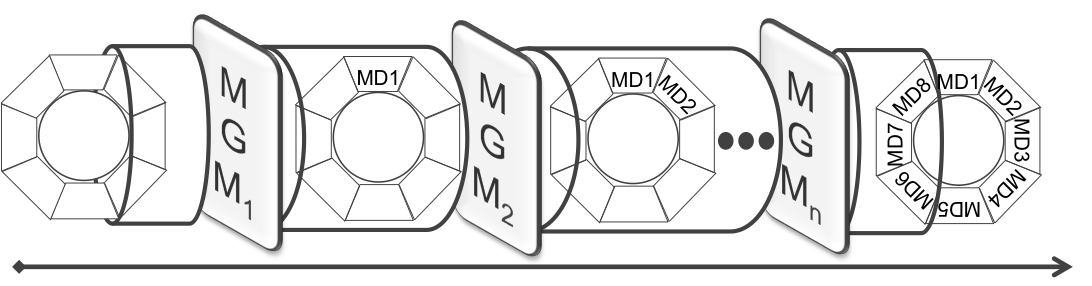
\includegraphics[width=\linewidth]{fig/md-pipe.png}
  \caption{Metadata Generation Pipeline}
  \label{fig:pipe}
\end{figure}

In this model the extraction or application steps in the pipeline are referred to as a \emph{\md{} generation module}, or MGM. As depicted in Figure \ref{fig:pipe}, a data object progresses through a series of MGMs, where an MGM comprises a script language specific to the task. At every stage a decision is made whether there is \md{} to be applied. While each MGM is independent, the ordering of MGMs can matter as the algorithm applied at any individual MGM may base a decision of whether to add, change or delete a \md{} section based not only the data object itself, but rather the union of the data object and \md{} accumulated in the pipeline to that point. Nonetheless, fundamental to this design is that an MGM is independent, to allow the flexibility of adding or updating MGMs in existing pipelines.

In HCP the address space is partitioned into \emph{namespaces} that essentially act as a virtual instance of the system as a whole. This segregation allows different data management and access policies to be applied to each set of data objects housed within a particular namespace.  It is a natural extension that each namespace may have a different set of MGMs to analyze data objects specific to a namespace (Figure \ref{fig:mgp}). This allows finer-grain decisions to applied to objects already grouped by user.

\begin{figure}[h]
  \centering
    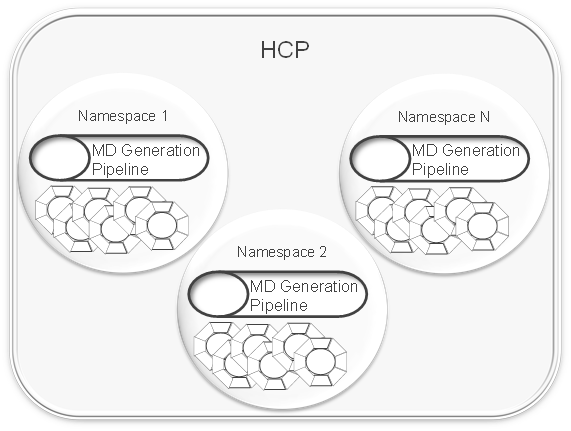
\includegraphics[width=\linewidth]{fig/cluster-mgp.png}
  \caption{Unique Pipeline per Namespace}
  \label{fig:mgp}
\end{figure}

Database programmers likely recognize that the MGM construct is conceptually similar to a \emph{stored procedure} in a RDBMS. A stored procedure is a subroutine stored in the \db{} data dictionary that runs on the \db{} server itself rather than directly on the client. In this model the MGM acts as a stored procedure, where common code can be run directly on the RDOS cluster rather than the client.

Note that a client \app{} could choose to perform all the functions of the MGM pipeline directly by reading an object, applying \md{}, and then rewriting this object back to the RDOS cluster. The downside of this method is that network bandwidth is consumed by the roundtrip for the read/write operations. It can therefore be more efficient to perform this same function on the cluster by running objects through the MGM pipeline. MGM scripts can be created either by the \app{} provider or constructed by the system administrator through a GUI.
